\documentclass[
  bibliography=totoc,     % Literatur im Inhaltsverzeichnis
  captions=tableheading,  % Tabellenüberschriften
  titlepage=firstiscover, % Titelseite ist Deckblatt
]{scrartcl}

% Paket float verbessern
\usepackage{scrhack}

% Warnung, falls nochmal kompiliert werden muss
\usepackage[aux]{rerunfilecheck}

% unverzichtbare Mathe-Befehle
\usepackage{amsmath}
% viele Mathe-Symbole
\usepackage{amssymb}
% Erweiterungen für amsmath
\usepackage{mathtools}

% Fonteinstellungen
\usepackage{fontspec}
% Latin Modern Fonts werden automatisch geladen
% Alternativ:
%\setromanfont{Libertinus Serif}
%\setsansfont{Libertinus Sans}
%\setmonofont{Libertinus Mono}
\recalctypearea % Wenn man andere Schriftarten gesetzt hat,
% sollte man das Seiten-Layout neu berechnen lassen

% deutsche Spracheinstellungen
\usepackage{polyglossia}
\setmainlanguage{german}


\usepackage[
  math-style=ISO,    % ┐
  bold-style=ISO,    % │
  sans-style=italic, % │ ISO-Standard folgen
  nabla=upright,     % │
  partial=upright,   % ┘
  warnings-off={           % ┐
    mathtools-colon,       % │ unnötige Warnungen ausschalten
    mathtools-overbracket, % │
},                       % ┘
]{unicode-math}

% traditionelle Fonts für Mathematik
\setmathfont{Latin Modern Math}
% Alternativ:
%\setmathfont{Libertinus Math}

\setmathfont{XITS Math}[range={scr, bfscr}]
\setmathfont{XITS Math}[range={cal, bfcal}, StylisticSet=1]

% Zahlen und Einheiten
\usepackage[
locale=DE,                   % deutsche Einstellungen
separate-uncertainty=true,   % immer Fehler mit \pm
per-mode=symbol-or-fraction, % / in inline math, fraction in display math
]{siunitx}

% chemische Formeln
\usepackage[
version=4,
math-greek=default, % ┐ mit unicode-math zusammenarbeiten
text-greek=default, % ┘
]{mhchem}

% richtige Anführungszeichen
\usepackage[autostyle]{csquotes}

% schöne Brüche im Text
\usepackage{xfrac}

% Standardplatzierung für Floats einstellen
\usepackage{float}
\floatplacement{figure}{htbp}
\floatplacement{table}{htbp}

% Floats innerhalb einer Section halten
\usepackage[
section, % Floats innerhalb der Section halten
below,   % unterhalb der Section aber auf der selben Seite ist ok
]{placeins}

% Seite drehen für breite Tabellen: landscape Umgebung
\usepackage{pdflscape}

% Captions schöner machen.
\usepackage[
  labelfont=bf,        % Tabelle x: Abbildung y: ist jetzt fett
  font=small,          % Schrift etwas kleiner als Dokument
  width=0.9\textwidth, % maximale Breite einer Caption schmaler
]{caption}
% subfigure, subtable, subref
\usepackage{subcaption}

% Grafiken können eingebunden werden
\usepackage{graphicx}
% größere Variation von Dateinamen möglich
\usepackage{grffile}

% schöne Tabellen
\usepackage{booktabs}

% Verbesserungen am Schriftbild
\usepackage{microtype}

% Literaturverzeichnis
\usepackage[style=alphabetic,]{biblatex}
% Quellendatenbank
\addbibresource{lit.bib}

% Hyperlinks im Dokument
\usepackage[
  unicode,        % Unicode in PDF-Attributen erlauben
  pdfusetitle,    % Titel, Autoren und Datum als PDF-Attribute
  pdfcreator={},  % ┐ PDF-Attribute säubern
  pdfproducer={}, % ┘
]{hyperref}
% erweiterte Bookmarks im PDF
\usepackage{bookmark}

% Trennung von Wörtern mit Strichen
\usepackage[shortcuts]{extdash}

\title{V703: Das Geiger-Müller-Zählrohr}
\author{
  Simon Schulte
  \texorpdfstring{
    \\
    \href{mailto:simon.schulte@udo.edu}{simon.schulte@udo.edu}
  }{}
  \texorpdfstring{\and}{, }
  Tim Sedlaczek
  \texorpdfstring{
    \\
    \href{mailto:tim.sedlaczek@udo.edu}{tim.sedlaczek@udo.edu}
  }{}
}
\publishers{TU Dortmund – Fakultät Physik}

\date{Durchführung: 18.04.2017\\
      Abgabe: 25.04.2017}


\begin{document}

\maketitle
\thispagestyle{empty}
\tableofcontents
\newpage
\setcounter{page}{1}
\section{Zielsetzung}
\label{sec:zielsetzung}
In diesem Versuch wird mit Hilfe eines Geiger-Müller-Zählrohrs die Intensität
ionisierender Strahlung gemessen.
\section{Theorie}
\label{sec:theorie}
Das Geiger-Müller-Zählrohr dient dazu, die Intensität ionisierender Strahlung
zu messen. Wenn nämlich ionisierende Strahlung in das Geiger-Müller-Zählrohr
eintritt, gibt das Zählrohr einen elektronischen Impuls ab, welcher leicht von
einem Impulsmesser wahrgenommen werden kann.
In Abbildung \ref{fig:V7031} zu sehen ist der schematische Aufbau eines
solchen Zählrohrs. Ein Zählrohr besteht aus einem Stahlmantel, in dessen
Mitte sich axial ein positiv geladener Anodendraht befindet. Der Anodendraht
leitet widerum die Betriebsspannung $U$. Diese ist nötig, um eine
Potentialdifferenz zwischen dem Mantel und dem Draht zu gewährleisten. Außerdem
ist eine Mylar-Folie am linken Ende des Zählrohrs befestigt, welche als
Eintrittsfenster dient. Diese gewährleistet, dass sogar $\alpha$-Strahlung in
das Rohr durchdringt, welche eigentlich schon von einem Stück Papier aufgehalten
wird. In diesem Versuch wird allerdings nur $\beta$-Strahlung (in Form von Elektronen)
betrachtet. Im Inneren des Zählrohrs ist ein Gasgemisch, welches hauptsächlich aus
Argon besteht. Das Gasgemisch hat den Zweck, dass, wenn ein geladenes Teilchen durch
das Eintrittsfenster dringt, sich dessen Energie durch Ionisation aufbraucht.
\begin{figure}[htb]
  \centering
  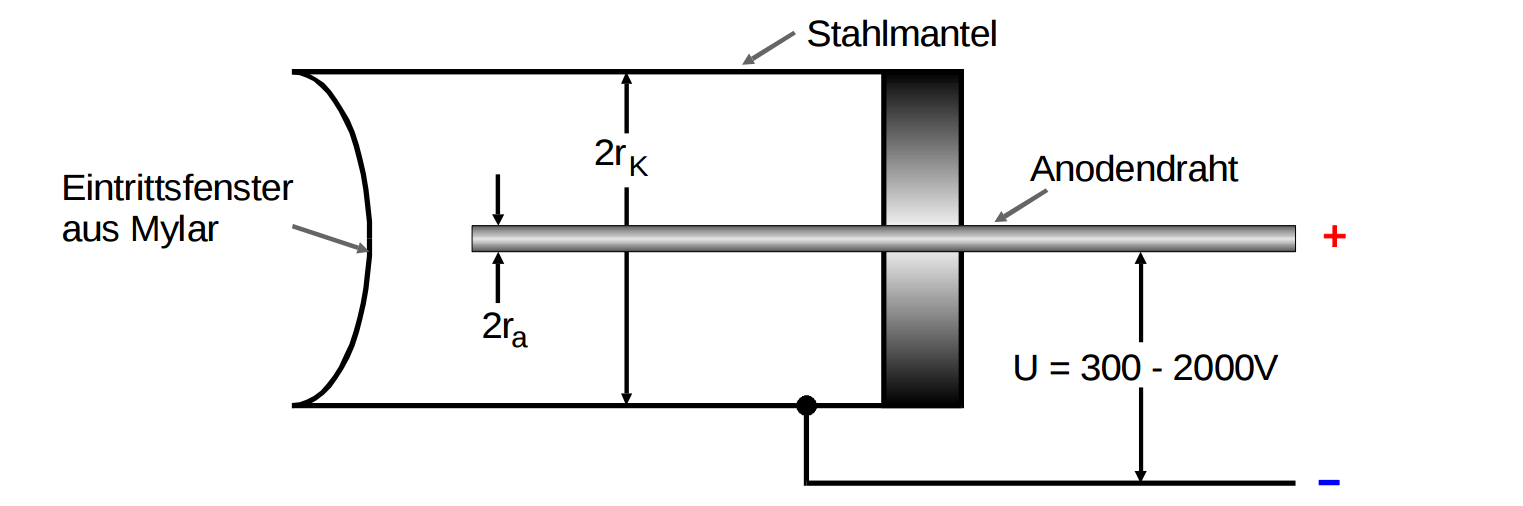
\includegraphics[width=0.9\textwidth]{V7031.png}
  \caption{Der Querschnitt eines Endfenster-Zählrohrs \cite{anleitung}.}
  \label{fig:V7031}
\end{figure}

\noindent
In Abbildung \ref{fig:V7032} zu sehen ist nun die Abhängigkeit der Anzahl der
erzeugten Ionenpaare von der Spannung $U$ bei einem Proportionalitätszählrohr.
So werden bei kleinen Betriebsspannungen nur wenige Elektronen den Draht
erreichen, da die meisten vorher rekombiniert werden. In der zweiten Zone, der
Ionisationskammer, können aufgrund der immer größer werdenden Spannung kaum noch
Elektronen rekombinieren, bevor sie den Anodendraht erreichen können. Damit
kommen fast alle Elektronen am Draht an. Diese erzeugen dann einen
Ionisationsstrom, der proportional zur Energie der ionisierenden Strahlung ist.
In der dritten Zone, dem (begrenzten) Proportionalbereich entsteht Stoßionisation.
Das heißt, dass die bei der Ionisation freigesetzten Elektronen vor dem Zusammenstoß
mit einem weiteren Atom aus dem Gasgemisch hinreichend viel Energie aufnehmen, um
selbst ionisieren zu können. Da diese Elektronen selbst immer wieder ionisieren
können, nimmt die Anzahl lawinenartig zu, auch Townsend-Lawine genannt.
In der vierten Zone beginnt dann der Arbeitsbereich des Geiger-Müller-Zählrohrs,
gennant Auslösebereich. Die Elektronenlawinen breiten sich nun nicht mehr nur,
wie in Zone 3, in Feldrichtung aus, sondern sind auch in der Lage den gesamten Draht
zu erreichen. Das liegt daran, dass bei der Ionisation nun auch neutral geladene
UV-Strahlung entsteht, welche ebenfalls Gas ionisieren kann und nicht an die elektrischen
Feldlinien gebunden ist. Dadurch entstehen elektrische Impulse, die dann groß genug
sind, um sie mit einem Impulszähler zu detektieren.
\begin{figure}[htb]
  \centering
  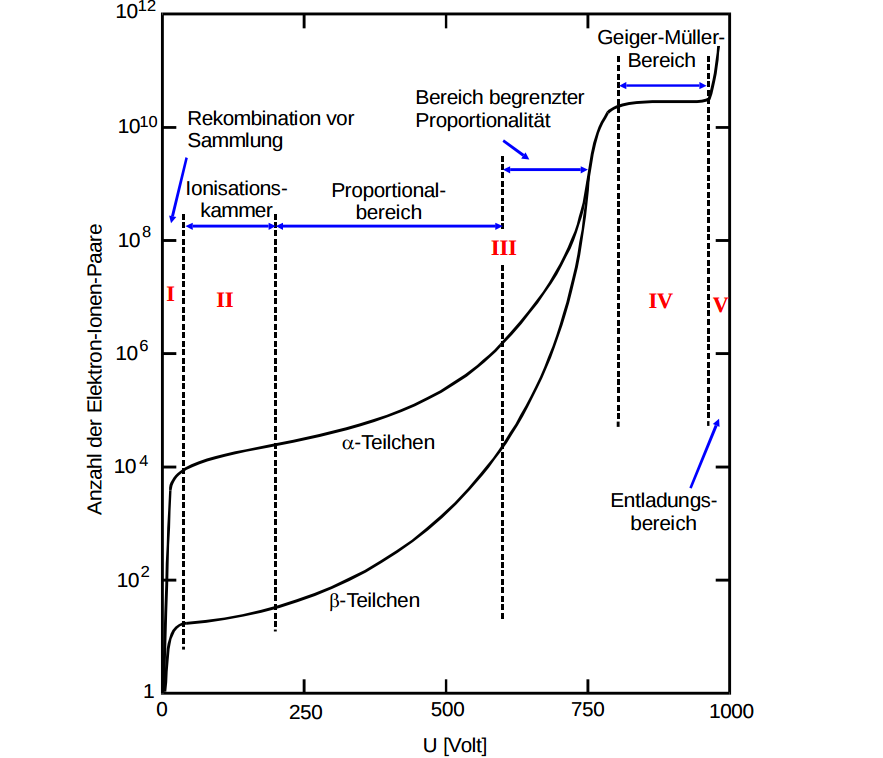
\includegraphics[width=0.9\textwidth]{V7032.png}
  \caption{Die Anzahl der erzeugten Elektron-Ionenpaare als Funktion der
  Spannung U bei einem Proportionalzählrohr \cite{anleitung}.}
  \label{fig:V7032}
\end{figure}

\noindent
In Abbildung \ref{fig:V7033} zu sehen ist nun die Tot- und Erholzeit des
Zählrohrs, wobei die Ladung als Funktion der Zeit dargestellt wird.
Da die positiven Ionen ein vielfaches der Masse der Elektronen besitzen
verschwinden diese auch langsamer. So bildet sich, in dem Zählrohr, zunächst ein
Ionenschlauch, welcher für ein Gegenfeld zum angelegten E-Feld sorgt. Dies führt dazu, dass das
Zählrohr in der Totzeit keine weitere $\beta$-Strahlung detektiert.
Nach der Totzeit stellt sich die Erholungszeit ein, in welcher widerum die
abgegebenen elektrischen Impulse des Rohrs kleiner ausfallen.
\clearpage
\begin{figure}[htb]
  \centering
  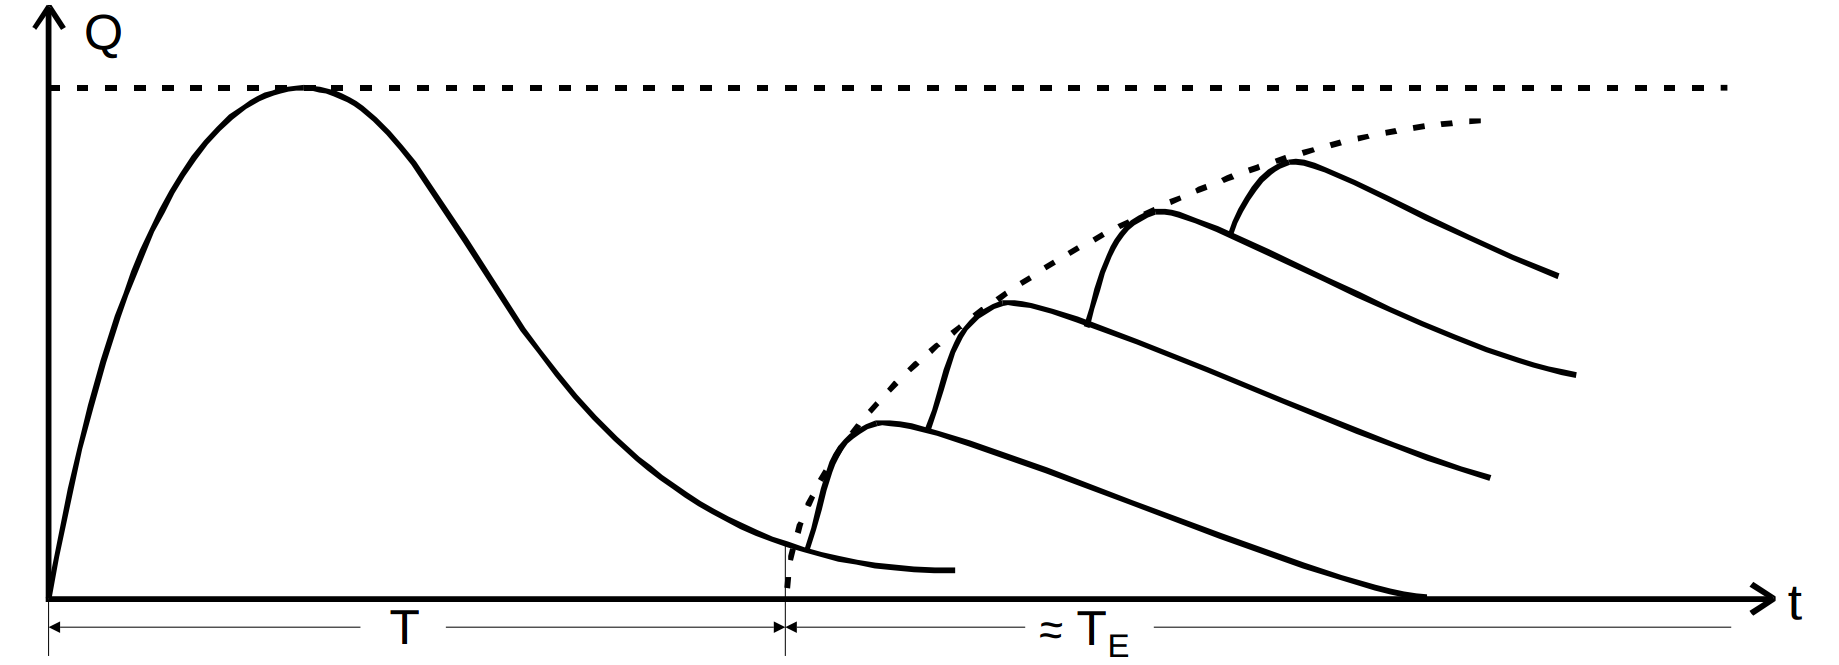
\includegraphics[width=0.9\textwidth]{V7033.png}
  \caption{Die Tot- und Erholungszeit eines Zählrohrs, dabei wird die Ladung Q
  als Funktion der Zeit abgebildet \cite{anleitung}.}
  \label{fig:V7033}
\end{figure}
\begin{figure}[htb]
  \centering
  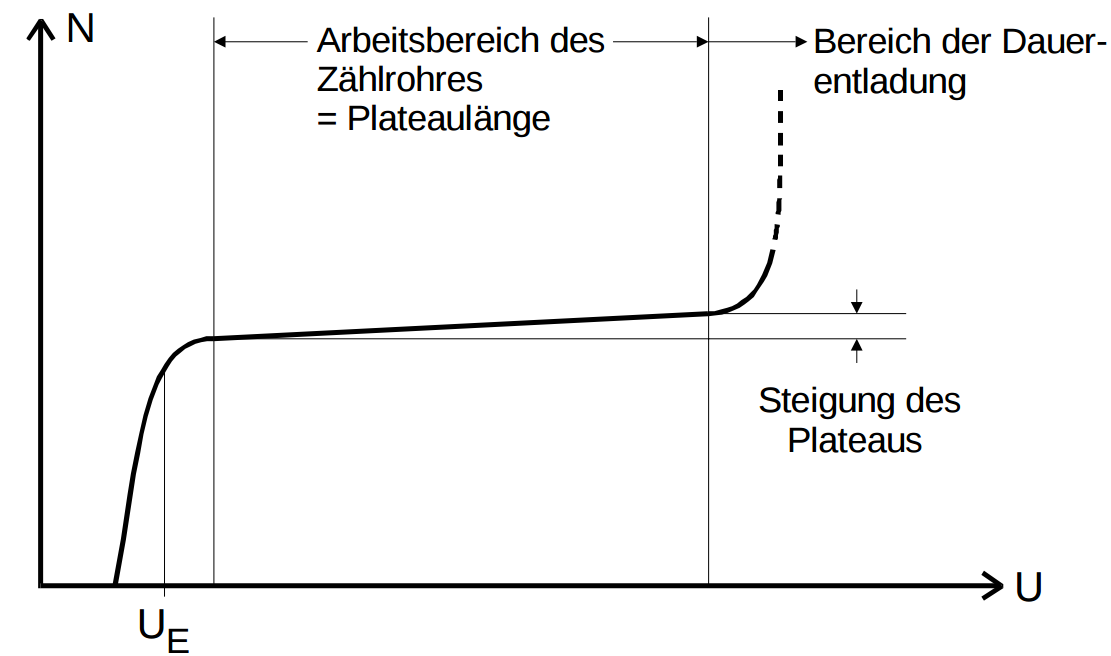
\includegraphics[width=0.9\textwidth]{V7034.png}
  \caption{Die Charakteristik eines Zählrohres \cite{anleitung}.}
  \label{fig:V7034}
\end{figure}

\noindent
In Abbildung \ref{fig:V7034} zu sehen ist die Charakteristik eines Zählrohres.
In der Charakteristik wird die Spannung $U$ gegen die im Zählrohr registrierte
Teilchenzahl $N$ aufgetragen. Dabei wird eine konstante $\beta$-Strahlungsquelle verwendet.
Besonders interessant ist das Plateau, welches in einem idealen Zählrohr
konstant wäre, aber aufgrund von Nachentladungen in der Realität leicht ansteigt.
Diese Nachentladungen entstehen, wenn die positiv geladenen Ionen große Energien
erreichen. Wenn sie dann an den Stahlmantel gelangen sind sie in der Lage
Elektronen aus dem Stahlmantel zu lösen. Dadurch wird die Messung verfälscht.
Dem wird entgegengewirkt, indem dem Zählrohrgasgemisch Alkohol hinzugegeben wird.
Alkoholmoleküle sind vielkettig und die überflüssige Energie der Ionen kann
somit in Form von Schwingungsenergie an die langen Alkoholmoleküle abgegeben werden.
Allerdings klappt dies auch nicht einwandfrei, weshalb sich ein nicht perfektes
Plateau ergibt.
\section{Durchführung}
\subsection{Versuchsaufbau}
\begin{figure}[htb]
  \centering
  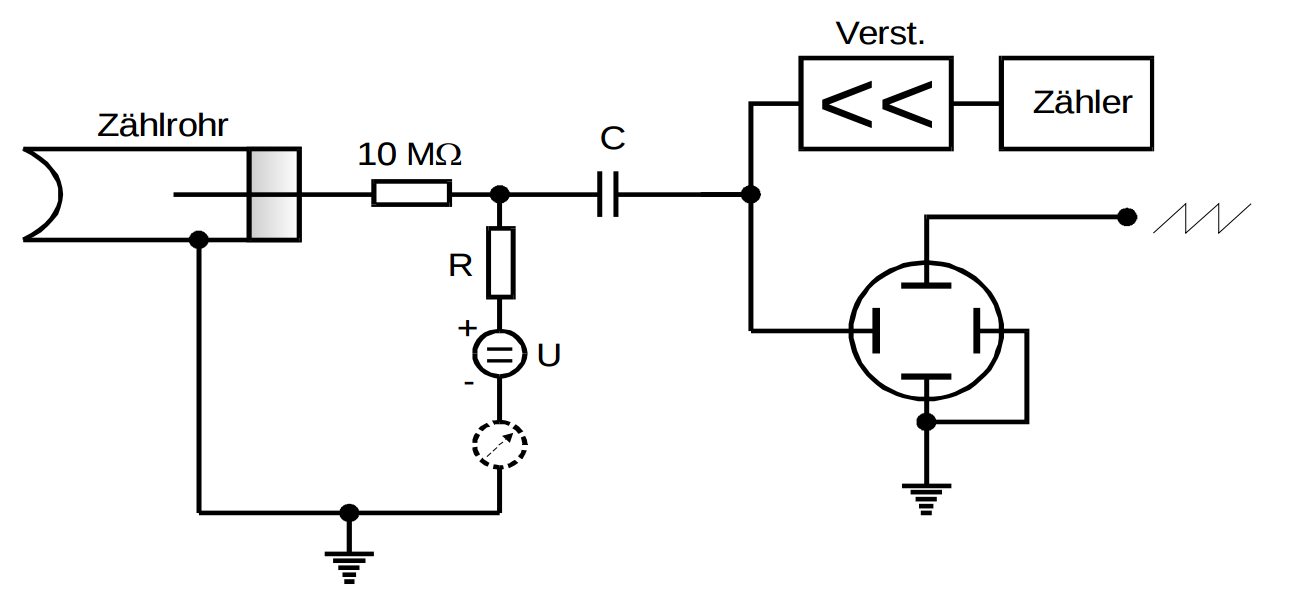
\includegraphics[width=0.9\textwidth]{V7035.png}
  \caption{Die Skizze der Messapparatur \cite{anleitung}.}
  \label{fig:V7035}
\end{figure}

\noindent
In Abbildung \ref{fig:V7035} zu sehen ist der Versuchsaufbau. Links ist das
Geiger-Müller-Zählrohr, mit dem Zähldraht, der mit einem
elektrischen Stromkreis verbunden ist. Die Ladungen der Elektronen werden dabei
auf dem Zähldraht gesammelt, um dann über den Widerstand $R$ zu fließen
und einen Spannungsimpuls zu verursachen. Dieser wird am Kondensator
ausgekoppelt und im Verstärker verstärkt. Der Zähler zählt dann die Anzahl
der Ereignisse. Das Oszilloskop wird zur Visualisierung genutzt.
\subsection{Versuchsablauf}
Um die Aufenthaltszeit zu minimieren werden Teil a) und Teil d) gleichzeitig
durchgeführt.

\noindent
In Teil a) soll eine Zählrohr-Charakteristik erstellt werden. Dafür wird eine
$\beta$-Quelle vor dem Mylar-Eintrittsfenster platziert und für die Werte
\SI{320}{\volt} bis \SI{700}{\volt} in Zehner Schritten jeweils für 60 Sekunden
die Zählrate gemessen.

\noindent
In Teil b) werden die Zeitpunkte der ersten beiden Nachentladungen für die
Maximalspannung von \SI{700}{\volt} bestimmt. Die Nachentladeimpulse werden am
Oszilloskop abgelesen.

\noindent
In Teil c) werden mit dem Oszilloskop die Totzeit und die Erholungszeit, für
verschiedene Spannungen, bestimmt. Hierzu werden, in \SI{20}{\volt} Abständen,
Spannungen zwischen \SI{400}{\volt} und \SI{500}{\volt} eingestellt, die in
der Mitte des Plateaus liegen.
Als zweite Messmethode, um die Totzeit zu bestimmen, werden, bei einer Spannung
von \SI{450}{\volt} (Plateaumitte), die Zählraten von 2 verschiedenen $\beta$-Strahlern,
einzeln und zusammen, gemessen. Hierbei ist darauf zu achten, dass sich die Positionen
der Quellen zwischen den Messungen nicht verändern. Zunächst wird also die erste
Quelle vermessen. Als Zweites Beide zusammen und schließlich nur die zweite Quelle.
Aus den verschiedenen Zählraten lässt sich dann die Totzeit bestimmen.

\noindent
In Teil d) wird der, von den Ionen erzeugte, Strom am Zählrohr gemessen und daraus,
unter Verwendung der Zählrate, die Ladung, die pro Teilchen im Zählrohr freigesetzt
wird, bestimmt.
\section{Auswertung}
\label{sec:auswertung}
\subsection{Zählrohrcharakteristik und pro Teilchen im Zählrohr freigesetzte Ladung}
Bei der Messung wurden die in Tabelle \ref{tab:charakter} stehenden Werte gemessen.
Zunächst soll die Zählrohr-Charakteristik erstellt werden.
Dafür werden die Zählraten in Ereignisse pro Sekunde umgerechnet und
der Fehler $\Delta n$ der einzelnen Messungen bestimmt.
Der Fehler berechnet sich dabei nach
\begin{equation}
  \Delta n = \frac{\sqrt{N}}{\SI{60}{\second}}.
\end{equation}
Diese Werte stehen ebenfalls in Tabelle \ref{tab:charakter} und sind in Abbildung \ref{fig:plot1} dargestellt.
Für den bereich zwischen \SI{370}{\volt} bis \SI{640}{\volt}, bei dem wir das
Plateau vermuten, wurde mittels Python eine Ausgleichsgerade der Form
\begin{equation}
  f(U) = A \cdot U + B
\end{equation}
erstellt.
Als Parameter ergeben sich dafür
\begin{align}
  A &= \SI{0.071\pm0.009}{\per\second\per\volt} & &\text{und} &B = \SI{437\pm4}{\per\second}
\end{align}
\begin{figure}
  \centering
  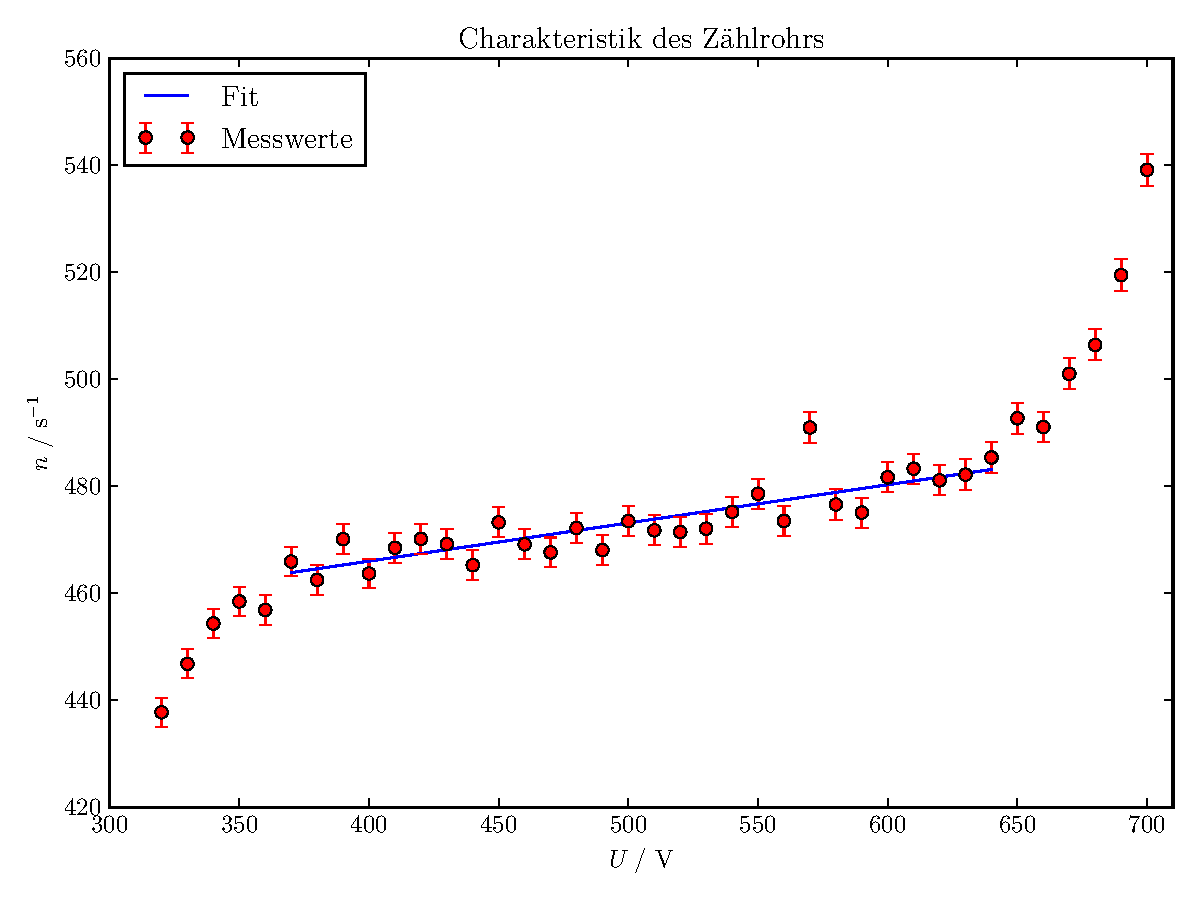
\includegraphics[width=0.74\textwidth]{Plot.pdf}
  \caption{Graph der Messwerte und der Ausgleichsgeraden zum Plateau.}
  \label{fig:plot1}
\end{figure}
\begin{table}
  \centering
  \caption{Zählrate und Strom bei entsprechender Spannung.}
  \label{tab:charakter}
  \sisetup{table-format=1.1}
  \begin{tabular}{S[table-format=3.0] S[table-format=5.0] S[table-format=3.0] S[table-format=1.0] S}
    \toprule
     {Angelegte Spannung $U$ in $\si{\volt}$} & {$N$ (pro $\SI{60}{\second}$)} & {$n$ (pro $\si{\second}$)} & {$\Delta n$ (pro $\si{\second}$)} & {Ladungsstrom $I$ in $\si{\micro\ampere}$} \\
    \midrule
    320 & 26263 & 438 & 3 & 0.3 \\
    330 & 26807 & 447 & 3 & 0.4 \\
    340 & 27259 & 454 & 3 & 0.5 \\
    350 & 27506 & 458 & 3 & 0.6 \\
    360 & 27412 & 457 & 3 & 0.7 \\
    370 & 27954 & 466 & 3 & 0.8 \\
    380 & 27748 & 462 & 3 & 0.9 \\
    390 & 28205 & 470 & 3 & 1.0 \\
    400 & 27820 & 464 & 3 & 1.1 \\
    410 & 28108 & 468 & 3 & 1.2 \\
    420 & 28208 & 470 & 3 & 1.3 \\
    430 & 28150 & 469 & 3 & 1.4 \\
    440 & 27913 & 465 & 3 & 1.5 \\
    450 & 28393 & 473 & 3 & 1.6 \\
    460 & 28147 & 469 & 3 & 1.7 \\
    470 & 28056 & 468 & 3 & 1.8 \\
    480 & 28331 & 472 & 3 & 1.9 \\
    490 & 28082 & 468 & 3 & 2.0 \\
    500 & 28407 & 473 & 3 & 2.1 \\
    510 & 28304 & 472 & 3 & 2.2 \\
    520 & 28286 & 471 & 3 & 2.3 \\
    530 & 28323 & 472 & 3 & 2.4 \\
    540 & 28511 & 475 & 3 & 2.5 \\
    550 & 28715 & 479 & 3 & 2.6 \\
    560 & 28409 & 473 & 3 & 2.7 \\
    570 & 29457 & 491 & 3 & 2.8 \\
    580 & 28594 & 477 & 3 & 2.9 \\
    590 & 28503 & 475 & 3 & 3.0 \\
    600 & 28899 & 482 & 3 & 3.1 \\
    610 & 28995 & 483 & 3 & 3.2 \\
    620 & 28865 & 481 & 3 & 3.2 \\
    630 & 28929 & 482 & 3 & 3.3 \\
    640 & 29121 & 485 & 3 & 3.4 \\
    650 & 29561 & 493 & 3 & 3.5 \\
    660 & 29463 & 491 & 3 & 3.6 \\
    670 & 30060 & 501 & 3 & 3.8 \\
    680 & 30384 & 506 & 3 & 3.9 \\
    690 & 31166 & 519 & 3 & 4.1 \\
    700 & 32348 & 539 & 3 & 4.2 \\
    \bottomrule
  \end{tabular}
\end{table}
\clearpage

\noindent
Zur Bestimmung der Steigung des Plateaus in \si{\percent} pro \SI{100}{\volt}
werden die Anfangs- und Endwerte
\begin{align}
  n_{370} &= \SI{463}{\per\second} & &\text{und} &n_{640} = \SI{482}{\per\second}
\end{align}
verwendet. Sie wurden mit der Ausgleichsfunktion bestimmt. Das Plateau ist etwa
\SI{270}{\volt} lang. Nach
\begin{equation}
  A_{\si{\percent}} = \frac{n_{640}-n_{370}}{n_{370}} \cdot \frac{100}{\SI{270}{\volt}}
\end{equation}
ergibt sich damit eine Steigung von
\begin{equation}
  A_{\si{\percent}} = \SI{1.5}{\percent} \; \text{pro} \; \SI{100}{\volt}.
\end{equation}\\
Die Stromstärke $I$ gibt die tranportierte Ladung
pro Zeit an. Um die freigesetzte Ladung pro Teilchen zu bestimmen, wird
sie mit dem Kehrwert der Zählrate multipliziert.
\begin{equation}
  \Delta Q = I \cdot \frac{1}{n}
\end{equation}
Zur Umrechnung in Vielfache der Elementarladung wird der bei Python im Paket Scientific Python
enthaltene Wert der Elementarladung verwendet. Dieser beträgt \SI{1.6021766208e-19}{\coulomb}
Die Ergebnisse stehen in Tabelle \ref{tab:ladung} und sind in Abbildung \ref{fig:plot2} dargestellt.
\begin{figure}
  \centering
  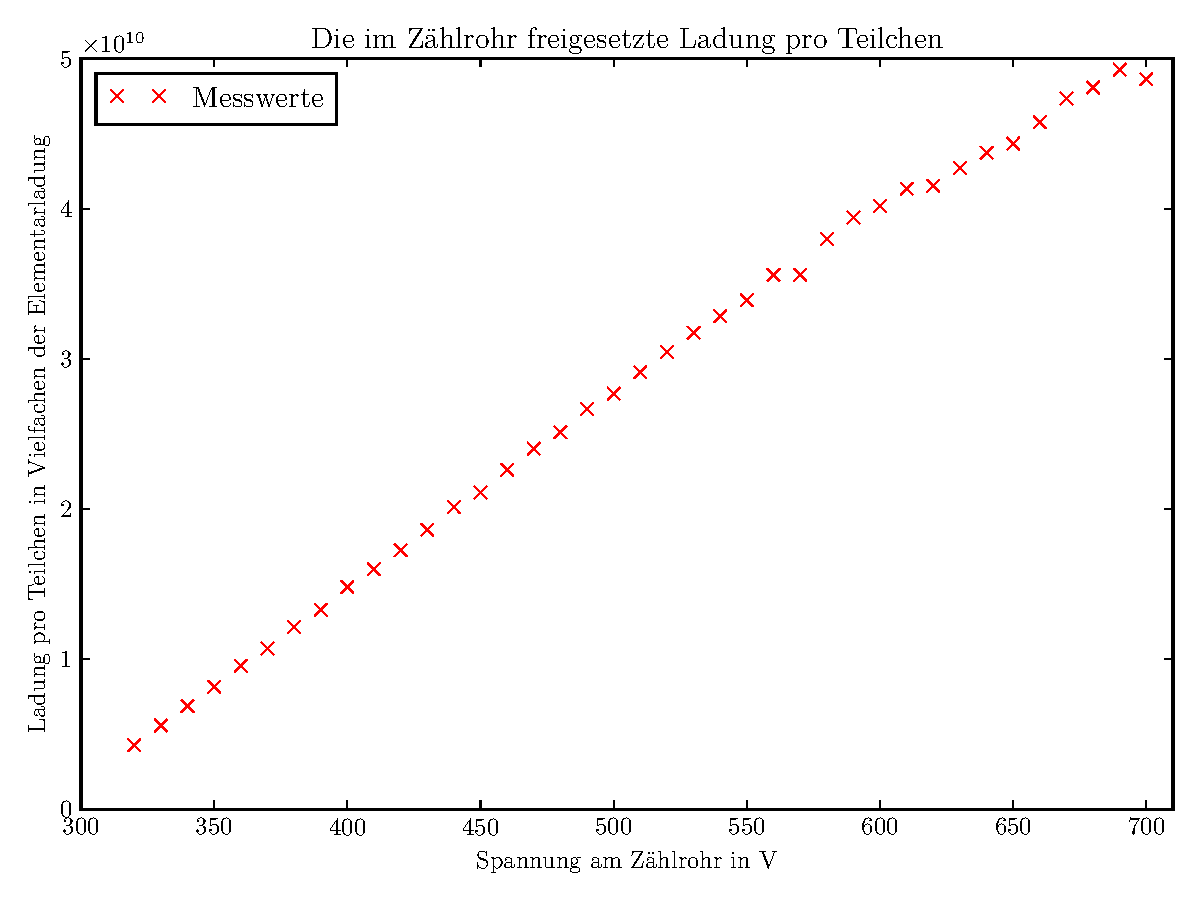
\includegraphics[width=0.8\textwidth]{Plot2.pdf}
  \caption{Freigesetzte Ladung bei der jeweiligen Spannung.}
  \label{fig:plot2}
\end{figure}
\begin{table}
  \centering
  \caption{Freigesetzte Ladung pro Teilchen.}
  \label{tab:ladung}
  \sisetup{table-format=1.1}
  \begin{tabular}{S[table-format=3.0] S[table-format=3.0] S S S}
    \toprule
      {Angelegte Spannung $U$} &  & {Ladungsstrom $I$} & \multicolumn{2}{c}{Freigesetzte Ladung pro Teilchen} \\
      {in $\si{\volt}$} & {$n$ (pro $\si{\second}$)} & {in $\si{\micro\ampere}$} & {in \si{\nano\coulomb}} & {in $\cdot 10^{10}$ Elementarladungen} \\
    \midrule
    320 & 438 & 0.3 & 0.7 & 0.4 \\
    330 & 447 & 0.4 & 0.9 & 0.6 \\
    340 & 454 & 0.5 & 1.1 & 0.7 \\
    350 & 458 & 0.6 & 1.3 & 0.8 \\
    360 & 457 & 0.7 & 1.5 & 1.0 \\
    370 & 466 & 0.8 & 1.7 & 1.1 \\
    380 & 462 & 0.9 & 1.9 & 1.2 \\
    390 & 470 & 1.0 & 2.1 & 1.3 \\
    400 & 464 & 1.1 & 2.4 & 1.5 \\
    410 & 468 & 1.2 & 2.6 & 1.6 \\
    420 & 470 & 1.3 & 2.8 & 1.7 \\
    430 & 469 & 1.4 & 3.0 & 1.9 \\
    440 & 465 & 1.5 & 3.2 & 2.0 \\
    450 & 473 & 1.6 & 3.4 & 2.1 \\
    460 & 469 & 1.7 & 3.6 & 2.3 \\
    470 & 468 & 1.8 & 3.8 & 2.4 \\
    480 & 472 & 1.9 & 4.0 & 2.5 \\
    490 & 468 & 2.0 & 4.3 & 2.7 \\
    500 & 473 & 2.1 & 4.4 & 2.8 \\
    510 & 472 & 2.2 & 4.7 & 2.9 \\
    520 & 471 & 2.3 & 4.9 & 3.0 \\
    530 & 472 & 2.4 & 5.1 & 3.2 \\
    540 & 475 & 2.5 & 5.3 & 3.3 \\
    550 & 479 & 2.6 & 5.4 & 3.4 \\
    560 & 473 & 2.7 & 5.7 & 3.6 \\
    570 & 491 & 2.8 & 5.7 & 3.6 \\
    580 & 477 & 2.9 & 6.1 & 3.8 \\
    590 & 475 & 3.0 & 6.3 & 3.9 \\
    600 & 482 & 3.1 & 6.4 & 4.0 \\
    610 & 483 & 3.2 & 6.6 & 4.1 \\
    620 & 481 & 3.2 & 6.7 & 4.2 \\
    630 & 482 & 3.3 & 6.8 & 4.3 \\
    640 & 485 & 3.4 & 7.0 & 4.4 \\
    650 & 493 & 3.5 & 7.1 & 4.4 \\
    660 & 491 & 3.6 & 7.3 & 4.6 \\
    670 & 501 & 3.8 & 7.6 & 4.7 \\
    680 & 506 & 3.9 & 7.7 & 4.8 \\
    690 & 519 & 4.1 & 7.9 & 4.9 \\
    700 & 539 & 4.2 & 7.8 & 4.9 \\
    \bottomrule
  \end{tabular}
\end{table}
\clearpage
\subsection{Zeitlicher Abstand zwischen Primär- und Nachentladungsimpuls}
Die Nachentladeimpulse waren am Oszilloskop sichtbar.
Der erste Nachentladeimuls fand \SI{125}{\micro\second} nach dem Primärimpuls
statt. Zum zweiten Nachentladeimpuls kam es \SI{200}{\micro\second} nach dem
Primärimpuls.
\subsection{Messung der Totzeit mit Hilfe eines Oszilloskops und mit Hilfe der Zwei-Quellen-Methode}
Mit dem Oszilloskop wurden die in Tabelle \ref{tab:totzeit} stehenden Werte
für die Totzeit und die Erholungszeit bestimmt.
\begin{table}
  \centering
  \caption{Tot- und Erholungszeit bei entsprechender Spannung.}
  \label{tab:totzeit}
  \sisetup{table-format=3.0}
  \begin{tabular}{S S S[table-format=4.0]}
    \toprule
     {Angelegte Spannung $U$ in $\si{\volt}$} & {Totzeit $T$ in $\si{\micro\second}$} & {Erholungszeit $T_E$ in $\si{\micro\second}$} \\
    \midrule
    400 & 125 & 1600 \\
    420 & 125 & 1500 \\
    440 & 125 & 1000 \\
    460 & 125 & 1400 \\
    480 & 125 & 1500 \\
    500 & 125 & 1400 \\
    \bottomrule
  \end{tabular}
\end{table}\\
Für die Erholungszeit wird der Mittelwert und der Standardfehler des Mittelwerts bestimmt.
Die Formel für den Standardfehler lautet:
\begin{equation}
  \Delta\overline{T_E} = \sqrt{\frac{1}{n(n-1)}\sum_{i=1}^n\left(T_{E.i}-\overline{T_E}\right)^2}.
  \label{eqn:standardabweichung}
\end{equation}
Damit ergibt sich eine mittlere Erholungszeit von \SI{1400(90)}{\micro\second}.\\

Mit der Zwei-Quellen-Methode wurden zunächst die in Tabelle \ref{tab:zweiquellen}
stehenden Zählraten gemessen. Die angelegte Spannung beträgt \SI{450}{\volt} und
die Fehler berechnen sich nach $\Delta N = \sqrt{N}$.
\begin{table}
  \centering
  \caption{Gemessene Zählraten bei der Zwei-Quellen-Methode.}
  \label{tab:zweiquellen}
  \sisetup{table-format=5.0}
  \begin{tabular}{S[table-format=3.0] S S[table-format=3.0]}
    \toprule
     {Quelle} & {Zählrate $N$ pro \SI{60}{\second}} & {Fehler $\Delta N$} \\
    \midrule
    1 & 19262 & 139 \\
    2 & 513 & 23 \\
    1$+$2 & 19539 & 140 \\
    \bottomrule
  \end{tabular}
\end{table}\\
\clearpage
\noindent
Mit der Anleitung \cite{anleitung} war für diese Methode die Formel
\begin{equation}
  \frac{N_{1+2}}{1-TN_{1+2}} = \frac{N_1}{1-TN_1} + \frac{N_2}{1-TN_2}
\end{equation}
gegeben. Durch Umformen und Lösen der quadratischen Gleichung ergibt sich:
\begin{equation}
  T = \frac{1}{N_{1+2}} \pm \sqrt{\frac{1}{N_{1+2}^2}-\biggl(\frac{1}{N_2N_{1+2}}+\frac{1}{N_1N_{1+2}}-\frac{1}{N_1N_2}\biggr)}
\end{equation}
Das negative Vorzeichen vor der Wurzel für zu keinem sinnvollen Ergebniss. Daher wird
es im Folgenden weggelassen.
Der Fehler dieser Größe wird mit Hilfe von Python über Fehlerfortpflanzung bestimmt.
Die Formel dafür ist:
\begin{align}
  \Delta T &= \sqrt{\biggl( \frac{\partial T}{\partial N_1} \cdot \Delta N_1 \biggr)^2+\biggl( \frac{\partial T}{\partial N_2} \cdot \Delta N_2 \biggr)^2+\biggl( \frac{\partial T}{\partial N_{1+2}} \cdot \Delta N_{1+2} \biggr)^2}\\
  \frac{\partial T}{\partial N_1} &= \frac{\frac{1}{N_1^2N_{1+2}}-\frac{1}{N_1^2N_2}}{2\sqrt{\frac{1}{N_{1+2}}-\frac{1}{N_1N_{1+2}}-\frac{1}{N_2N_{1+2}}+\frac{1}{N_1N_2}}}\\
  \frac{\partial T}{\partial N_2} &= \frac{\frac{1}{N_2^2N_{1+2}}-\frac{1}{N_1N_2^2}}{2\sqrt{\frac{1}{N_{1+2}}-\frac{1}{N_1N_{1+2}}-\frac{1}{N_2N_{1+2}}+\frac{1}{N_1N_2}}}\\
  \frac{\partial T}{\partial N_{1+2}} &= \frac{\frac{1}{N_1N_{1+2}^2}+\frac{1}{N_2N_{1+2}^2}-\frac{2}{N_{1+2}^3}}{2\sqrt{\frac{1}{N_{1+2}}-\frac{1}{N_1N_{1+2}}-\frac{1}{N_2N_{1+2}}+\frac{1}{N_1N_2}}} - \frac{1}{N_{1+2}^2}
\end{align}
Schließlich ergibt sich darüber eine Totzeit von
\begin{equation}
  T = \SI{89(13)}{\second}.
\end{equation}
\newpage
\section{Diskussion}
\label{sec:diskussion}
Die Messmethode mit dem Geiger-Müller-Zählrohr wirkt zuverlässig.

\noindent
In Teil a) ergibt sich ein insgesamt lineares Plateau mit leichten Schwankungen,
die allerdings überwiegend im Rahmen der Messfehler liegen.

\noindent
Bei Teil b) konnten Nachentladungen nachgewiesen werden, die für die Steigung
des Plateaus verantwortlich sind.

\noindent
In Teil c) wurde mit dem Oszilloskop eine Totzeit von \SI{125}{\micro\second} bestimmt
während bei der Zwei-Quellen-Methode sich eine Totzeit von \SI{89(13)}{\micro\second}
ergab. Die Totzeiten von Geiger-Müller-Zählrohren liegen in der Regel im Bereich
von \SI{100}{\micro\second} \cite{geigerwiki}.
Zu unserer Messung ist zu erwähnen, dass die Totzeit, am Oszilloskop, anhand vom ersten
Peak (dem ersten Nachentladungs-Peak) bestimmt wurde. Tatsächlich ist, wie in Abbildung
\ref{fig:V7033} zu sehen ist, die Totzeit etwas kleiner. Der Wert der Zwei-Quellen-Methode
passt ebenfalls sehr gut, wobei das Ergebniss schnell abgefälscht werden kann, wenn die
Positionen der Quellen ein wenig verändert werden.
Richtig ausgeführt ergibt sich bei beiden Methoden eine gute Näherung für
die Totzeit.

\noindent
Bei Teil d) ergeben sich freigesetzte Ladungen in der Größenordnung von $10^{10}$.
Das Passt zu den Werten, die Abbildung \ref{fig:V7032} entnommen werden können.
\nocite{*}
\printbibliography
\end{document}
